%%%%%%%%%%%%%%%%%%%%%%%%%%% asme2e.tex %%%%%%%%%%%%%%%%%%%%%%%%%%%%%%%
% Template for producing ASME-format articles using LaTeX            %
% Written by   Harry H. Cheng                                        %
%              Integration Engineering Laboratory                    %
%              Department of Mechanical and Aeronautical Engineering %
%              University of California                              %
%              Davis, CA 95616                                       %
%              Tel: (530) 752-5020 (office)                          %
%                   (530) 752-1028 (lab)                             %
%              Fax: (530) 752-4158                                   %
%              Email: hhcheng@ucdavis.edu                            %
%              WWW:   http://iel.ucdavis.edu/people/cheng.html       %
%              May 7, 1994                                           %
% Modified: February 16, 2001 by Harry H. Cheng                      %
% Modified: January  01, 2003 by Geoffrey R. Shiflett                %
% Use at your own risk, send complaints to /dev/null                 %
%%%%%%%%%%%%%%%%%%%%%%%%%%%%%%%%%%%%%%%%%%%%%%%%%%%%%%%%%%%%%%%%%%%%%%

%%% use twocolumn and 10pt options with the asme2e format
\documentclass[twocolumn,10pt]{asme2e}
\special{papersize=8.5in,11in}
\usepackage{graphicx}
\usepackage{caption}
\usepackage{subcaption}

%% The class has several options
%  onecolumn/twocolumn - format for one or two columns per page
%  10pt/11pt/12pt - use 10, 11, or 12 point font
%  oneside/twoside - format for oneside/twosided printing
%  final/draft - format for final/draft copy
%  cleanfoot - take out copyright info in footer leave page number
%  cleanhead - take out the conference banner on the title page
%  titlepage/notitlepage - put in titlepage or leave out titlepage
%  
%% The default is oneside, onecolumn, 10pt, final

%%% Replace here with information related to your conference
\confshortname{FEDSM 2020}
\conffullname{the ASME 2020 Fluids Engineering Division’s Summer Meeting}

%%%%% for date in a single month, use
%\confdate{24-28}
%\confmonth{September}
%%%%% for date across two months, use
\confdate{July 12-16}
\confyear{2020}
\confcity{Orlando}
\confcountry{USA}

%%% Replace DETC2009/MESA-12345 with the number supplied to you 
%%% by ASME for your paper.
\papernum{FEDSM2020-12388}

%%% You need to remove 'DRAFT: ' in the title for the final submitted version.
\title{DRAFT: The Effect of Variying Viscosity in Turbulent Channel Flow}
%%% for the discussion section only
%\usepackage{helvet}
%\title{\fontfamily{phv}\selectfont{\Huge{DRAFT: AN ARTICLE CREATED USING \LaTeX2\raisebox{-.3ex}{$\epsilon$}\ IN ASME FORMAT}}}

%%% first author
\author{Victor Coppo Leite
    \affiliation{
	Ken and Mary Alice Lindquist\\Department of Nuclear Engineering\\
	Pennsylvania State University\\
	State College, PA 16801\\
    Email: vbc5085@psu.edu
    }	
}

%%% second author
%%% remove the following entry for single author papers
%%% add more entries for additional authors
\author{Elia Merzari
    \affiliation{
	Ken and Mary Alice Lindquist\\Department of Nuclear Engineering\\
	Pennsylvania State University\\
	State College, PA 16801\\
    Email: ebm5153@psu.edu
    }	
}

\begin{document}

\maketitle    

%%%%%%%%%%%%%%%%%%%%%%%%%%%%%%%%%%%%%%%%%%%%%%%%%%%%%%%%%%%%%%%%%%%%%%
\begin{abstract}
{\it In various applications in nuclear engineering and in particular in test reactors, heat removal is carried by single-phase axial flow. In these applications, we observe sharp changes in molecular viscosity while the density presents very limited changes. As a consequence, the Reynolds number increases often by 2-3 folds across the channel, with an inlet value often transitional.  In these conditions, turbulence changes significantly across the length of the channel with redistribution and thinning of the boundary layers. This is different from acceleration as the effect of changes in density is negligible. We aim to characterize in detail this phenomenon. 

In particular Nek5000, a spectral-element computational fluid dynamics (CFD) code, will be used to perform DNS of fluid flow in the transition regime for channel flow with varying viscosity.  We set up a novel benchmark case: the channel is extended in the stream-wise direction up to 20pi. The viscosity is kept constant in the first 4pi region. This inlet region is used as a cyclic region to obtain a fully developed flow profile at the beginning of the ramping region. The ramping region (4pi -20pi) is defined as a transition region where the viscosity is linearly decreased along the channel. The flow is homogenous in the span-wise direction due to the periodic boundary conditions. Due to the cyclic and wall boundary conditions, the flow is non-homogenous in the stream-wise and wall-normal direction respectively.

In this study, specific focus is given to the investigation of turbulence properties and structures in the near-wall region along the flow direction. Detailed turbulence budgets are collected and investigated. As expected, the results show that variation in the Reynolds across a channel does not cause an immediate change in the size of turbulent structures in the ramp region and a delay is in fact observed. Moreover, the results from the present study are compared with a correlation available in the literature for the friction velocity and as a function of the Reynolds-number.}
\end{abstract}

%%%%%%%%%%%%%%%%%%%%%%%%%%%%%%%%%%%%%%%%%%%%%%%%%%%%%%%%%%%%%%%%%%%%%%
\begin{nomenclature}
\entry{A}{You may include nomenclature here.}
\entry{$\alpha$}{There are two arguments for each entry of the nomemclature environment, the symbol and the definition.}
\end{nomenclature}

The spacing between abstract and the text heading is two line spaces.  The primary text heading is  boldface in all capitals, flushed left with the left margin.  The spacing between the  text and the heading is also two line spaces.

%%%%%%%%%%%%%%%%%%%%%%%%%%%%%%%%%%%%%%%%%%%%%%%%%%%%%%%%%%%%%%%%%%%%%%
\section*{INTRODUCTION}

The turbulence channel simulated is shown in Fig.~\ref{fig:geometries}. In this figure, regions I, II and III are defined by two planes crossing the channel. In this problem, the viscosity is a function of the streamwise distance, expressed here by the spatial variable \(x\). This parameter has constants values of \(1E-4\) Pa.s and \(5E-5\) Pa.s along regions I and III respectively, while in region II it decreases with respect to the inverse of \(x\).

For the present work, three cases varying the length of region II are studied. Cases I, II and III have their region II begining at \(x=4\pi\) and the length of region II are respectively \(16\pi\), \(8\pi\) and \(4\pi\). Fig.~\ref{fig:viscosity_cases} shows the plot of the viscosity as a function of \(x\) for each one of these cases. For all cases the inleat flow in region I is considered to be fully developed with \(Re_{\tau}=550\), i.e., the same conditions as in \cite{hoyas2008}, while a periodic condition is considered for the boundaries of the spamwise direction, i.e., \(z\) axis, and finally wall conditions are considered for the boudaries of the vertical direction, i.e., \(y\) axis.

\begin{figure}[!htbp]
	\centering
	\begin{subfigure}{0.4\textwidth} % width of left subfigure
		\includegraphics[width=\textwidth]{turbchannel_a.png}
		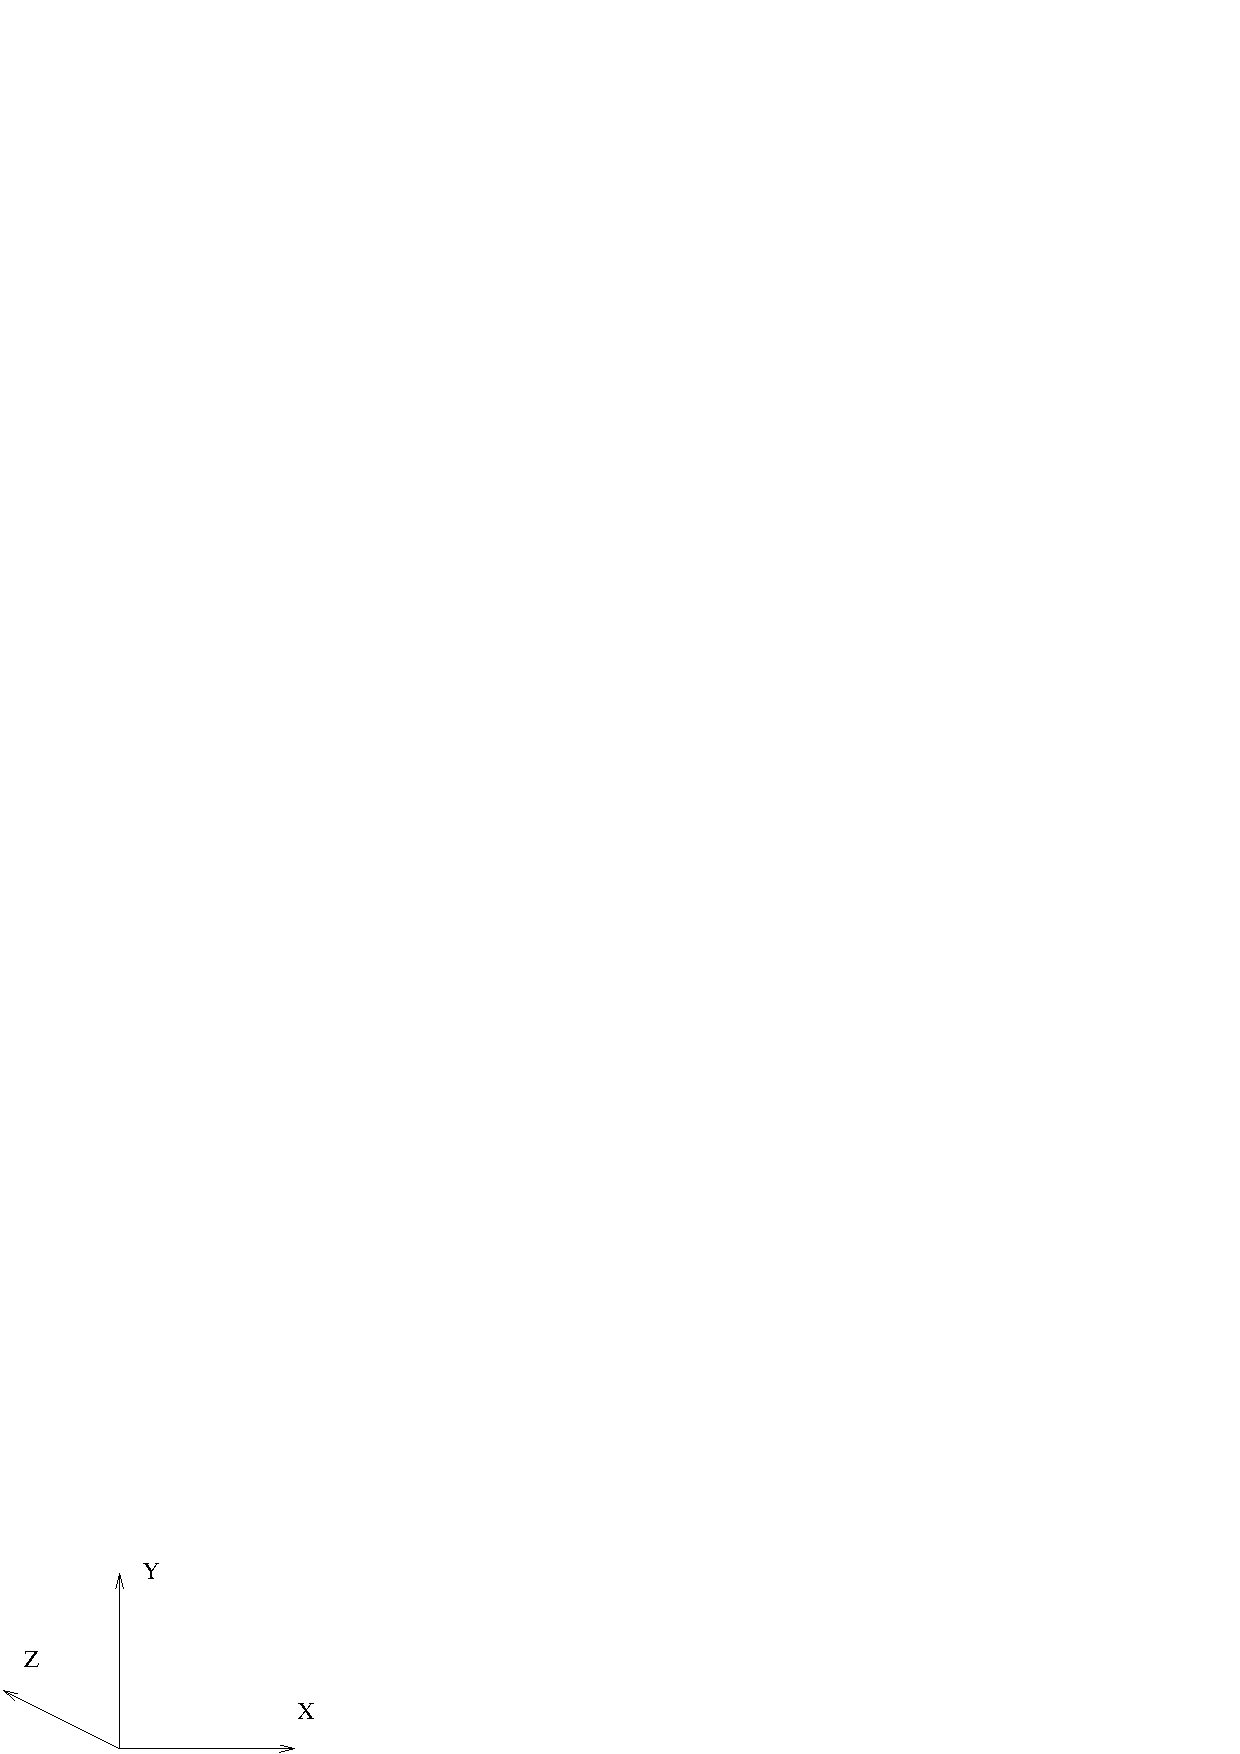
\includegraphics[trim = 0mm 0mm 0mm 20mm, width = 15mm]{axis.png}
		\caption{GEOMETRY OF THE TURBULENCE CHANNEL, THE CHANNEL IS DIVIDED INTO THREE DIFFERENT REGIONS.} % subcaption
	\label{fig:geometries}
	\end{subfigure}

	\begin{subfigure}{0.4\textwidth} % width of right subfigure
		\includegraphics[width=\textwidth]{turbchannel_b.png}
		\label{fig:cyclic_inlet}
		\caption{CYCLIC REGION IN THE INLET.} % subcaption
	\end{subfigure}
	\caption{SCHEMATICS OF THE SIMULATIONS EMPLOYED.} % caption for whole figure
	\label{fig:models}
\end{figure}

\begin{figure}[!htbp]
\begin{center}
\setlength{\unitlength}{0.012500in}%
  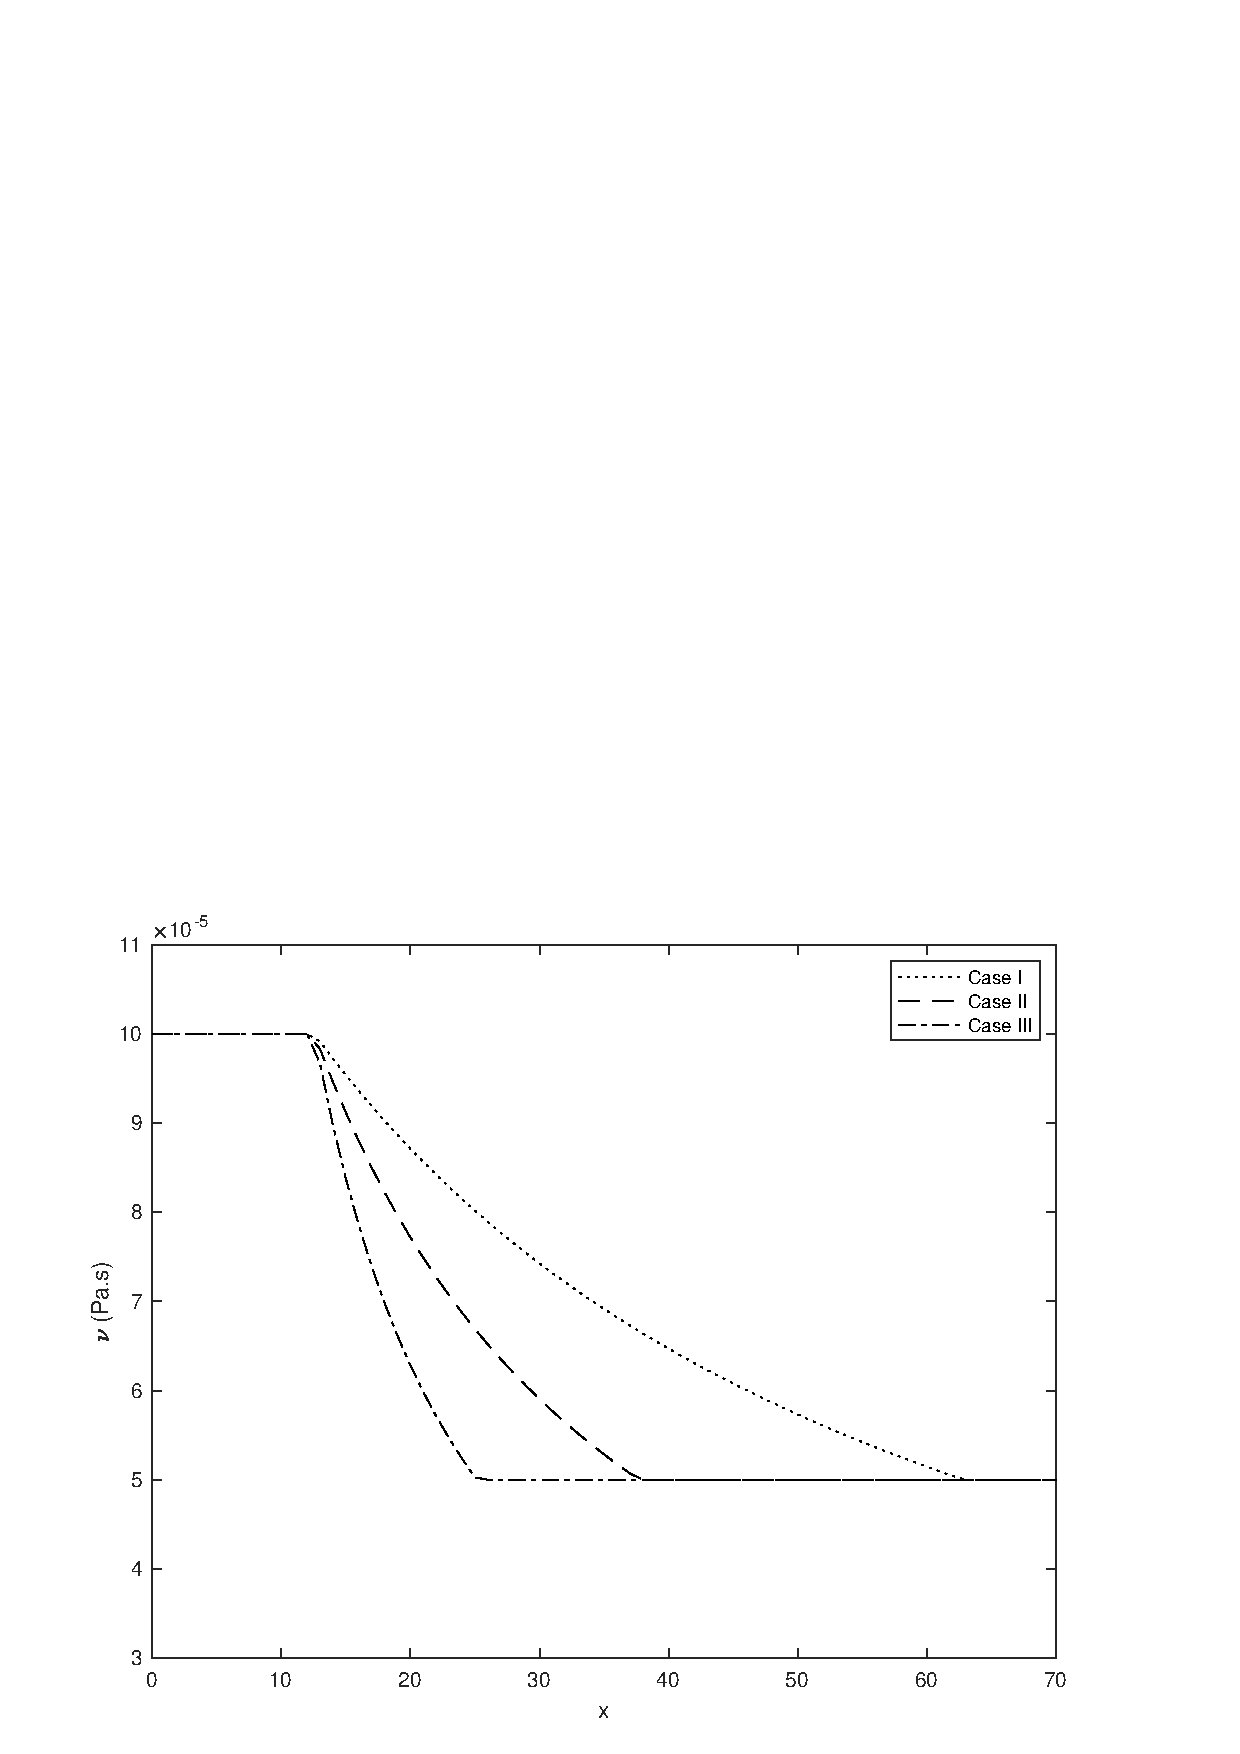
\includegraphics[trim = 20mm 15mm 30mm 10mm, width = 85mm]{viscosity.png}
\end{center}
  \caption{THE GRID EMPLOYED IN THE SIMULATION FROM HALF OF THE CHANNEL'S CROSS SECTION.}
  \label{fig:viscosity_cases}
\end{figure}


%%%%%%%%%%%%%%%%%%%%%%%%%%%%%%%%%%%%%%%%%%%%%%%%%%%%%%%%%%%%%%%%%%%%%%
\section*{METHODS}

In order to resolve the finest turbulent scales, the calculations of this work has been developed through Direct Numerical Simulation (DNS). To do so, a spectral element code Nek5000 was employed, where this code has been developed in Argonne National aboratory (ANL) and it has been validated in references \cite{merzari2013} and \cite{Obabko2011}.

The solution of this method is given by trigonometric series, in each element a polynomial functions of up to the twelveth degree have been employed to discretize the velocity field. Fig.~\ref{fig:cross_grid} shows an example of the grid from half of the channel's cross section. One should notice that the discretization presented by this particular area is identical through all model's domain and it is only presented half of the cross-section for better visualization of the frame.

\begin{figure}[!htbp]
\begin{center}
\setlength{\unitlength}{0.012500in}%
  \includegraphics[trim = 20mm 15mm 20mm 10mm, width = 90mm]{half_cross_section_mesh.png}
\end{center}
  \caption{THE GRID EMPLOYED IN THE STREAMWISE-DIRECTION CROSS SECTION OF THE TUBULENCE CHANNEL.}
  \label{fig:cross_grid}
\end{figure}

DNS simulations are able to simulate the finest turbulent length scales without using any turbulent model. Since the present work is focused on studying the contribution of the smaller scales to the energy cascade, it is required to use DNS rather than Reynolds Average Navier-Stokes (RANS) or Large Eddy Simulations (LES), although there is a substantial growth of the computational cost.

\underline{Add some stuff about the mesh and polynomial order.}



%%%%%%%%%%%%%%%%%%%%%%%%%%%%%%%%%%%%%%%%%%%%%%%%%%%%%%%%%%%%%%%%%%%%%%

\section*{RESULTS}

The results from the three cases considered in this work are presented in this section. First, the friction Reynolds number variation along the streamwise direction \(x\) of the channels are computed and compared with an expression for \(Re_{\tau}\) as a function of the Reynolds number existed in Ref.~\cite{pope}. This analysis shows the fact that the predicted shift in the friction Reynolds number due to a viscosity change imposed through region II is not immediate. Thereon, Reynolds stresses are collected and turbulent structures are investigated along the simulated channels.

%%%%%%%%%%%%%%%%%%%%%%%%%%%%%%%%%%%%%%%%%%%%%%%%%%%%%%%%%%%%%%%%%%%%%%

\subsection*{Analysing the friction Reynolds number}

Here goes nice things.

\subsection*{Reynolds stresses and turbulent structures}

More good stuff.



%%%%%%%%%%%%%%%%%%%%%%%%%%%%%%%%%%%%%%%%%%%%%%%%%%%%%%%%%%%%%%%%%%%%%%
\section*{USE OF SI UNITS}

An ASME paper should use SI units.  When preference is given to SI units, the U.S. customary units may be given in parentheses or omitted. When U.S. customary units are given preference, the SI equivalent {\em shall} be provided in parentheses or in a supplementary table. 

%%%%%%%%%%%%%%%%%%%%%%%%%%%%%%%%%%%%%%%%%%%%%%%%%%%%%%%%%%%%%%%%%%%%%%
\section*{MATHEMATICS}

Equations should be numbered consecutively beginning with (1) to the end of the paper, including any appendices.  The number should be enclosed in parentheses and set flush right in the column on the same line as the equation.  An extra line of space should be left above and below a displayed equation or formula. \LaTeX\ can automatically keep track of equation numbers in the paper and format almost any equation imaginable. An example is shown in Eqn.~(\ref{eq_ASME}). The number of a referenced equation in the text should be preceded by Eqn.\ unless the reference starts a sentence in which case Eqn.\ should be expanded to Equation.

\begin{equation}
f(t) = \int_{0_+}^t F(t) dt + \frac{d g(t)}{d t}
\label{eq_ASME}
\end{equation}

%%%%%%%%%%%%%%%%%%%%%%%%%%%%%%%%%%%%%%%%%%%%%%%%%%%%%%%%%%%%%%%%%%%%%%
\section*{FIGURES AND TABLES}

All figures should be positioned at the top of the page where possible.  All figures should be numbered consecutively and captioned; the caption uses all capital letters, and centered under the figure as shown in Fig.~\ref{figure_ASME}. All text within the figure should be no smaller than 7~pt. There should be a minimum two line spaces between figures and text. The number of a referenced figure or table in the text should be preceded by Fig.\ or Tab.\ respectively unless the reference starts a sentence in which case Fig.\ or Tab.\ should be expanded to Figure or Table.


%%%%%%%%%%%%%%%%%%%%%%%%%%%%%%%%%%%%%%%%%%%%%%%%%%%%%%%%%%%%%%%%%%%%%%
%%%%%%%%%%%%%%%% begin figure %%%%%%%%%%%%%%%%%%%
\begin{figure}[t]
\begin{center}
\setlength{\unitlength}{0.012500in}%
\begin{picture}(115,35)(255,545)
\thicklines
\put(255,545){\framebox(115,35){}}
\put(275,560){Beautiful Figure}
\end{picture}
\end{center}
\caption{THE FIGURE CAPTION USES CAPITAL LETTERS.}
\label{figure_ASME} 
\end{figure}
%%%%%%%%%%%%%%%% end figure %%%%%%%%%%%%%%%%%%% 
%%%%%%%%%%%%%%%%%%%%%%%%%%%%%%%%%%%%%%%%%%%%%%%%%%%%%%%%%%%%%%%%%%%%%%


%%%%%%%%%%%%%%%%%%%%%%%%%%%%%%%%%%%%%%%%%%%%%%%%%%%%%%%%%%%%%%%%%%%%%%
%%%%%%%%%%%%%%% begin table   %%%%%%%%%%%%%%%%%%%%%%%%%%
\begin{table}[t]
\caption{THE TABLE CAPTION USES CAPITAL LETTERS, TOO.}
\begin{center}
\label{table_ASME}
\begin{tabular}{c l l}
& & \\ % put some space after the caption
\hline
Example & Time & Cost \\
\hline
1 & 12.5 & \$1,000 \\
2 & 24 & \$2,000 \\
\hline
\end{tabular}
\end{center}
\end{table}
%%%%%%%%%%%%%%%% end table %%%%%%%%%%%%%%%%%%% 
%%%%%%%%%%%%%%%%%%%%%%%%%%%%%%%%%%%%%%%%%%%%%%%%%%%%%%%%%%%%%%%%%%%%%%

All tables should be numbered consecutively and  captioned; the caption should use all capital letters, and centered above the table as shown in Table~\ref{table_ASME}. The body of the table should be no smaller than 7 pt.  There should be a minimum two line spaces between tables and text.

%%%%%%%%%%%%%%%%%%%%%%%%%%%%%%%%%%%%%%%%%%%%%%%%%%%%%%%%%%%%%%%%%%%%%%
\section*{FOOTNOTES\protect\footnotemark}
\footnotetext{Examine the input file, asme2e.tex, to see how a footnote is given in a head.}

Footnotes are referenced with superscript numerals and are numbered consecutively from 1 to the end of the paper\footnote{Avoid footnotes if at all possible.}. Footnotes should appear at the bottom of the column in which they are referenced.


%%%%%%%%%%%%%%%%%%%%%%%%%%%%%%%%%%%%%%%%%%%%%%%%%%%%%%%%%%%%%%%%%%%%%%
\section*{CITING REFERENCES}

%%%%%%%%%%%%%%%%%%%%%%%%%%%%%%%%%%%%%%%%%%%%%%%%%%%%%%%%%%%%%%%%%%%%%%
The ASME reference format is defined in the authors kit provided by the ASME.  The format is:

\begin{quotation}
{\em Text Citation}. Within the text, references should be cited in  numerical order according to their order of appearance.  The numbered reference citation should be enclosed in brackets.
\end{quotation}

The references must appear in the paper in the order that they were cited.  In addition, multiple citations (3 or more in the same brackets) must appear as a `` [1-3]''.  A complete definition of the ASME reference format can be found in the  ASME manual \cite{asmemanual}.

The bibliography style required by the ASME is unsorted with entries appearing in the order in which the citations appear. If that were the only specification, the standard {\sc Bib}\TeX\ unsrt bibliography style could be used. Unfortunately, the bibliography style required by the ASME has additional requirements (last name followed by first name, periodical volume in boldface, periodical number inside parentheses, etc.) that are not part of the unsrt style. Therefore, to get ASME bibliography formatting, you must use the \verb+asmems4.bst+ bibliography style file with {\sc Bib}\TeX. This file is not part of the standard BibTeX distribution so you'll need to place the file someplace where LaTeX can find it (one possibility is in the same location as the file being typeset).

With \LaTeX/{\sc Bib}\TeX, \LaTeX\ uses the citation format set by the class file and writes the citation information into the .aux file associated with the \LaTeX\ source. {\sc Bib}\TeX\ reads the .aux file and matches the citations to the entries in the bibliographic data base file specified in the \LaTeX\ source file by the \verb+\bibliography+ command. {\sc Bib}\TeX\ then writes the bibliography in accordance with the rules in the bibliography .bst style file to a .bbl file which \LaTeX\ merges with the source text.  A good description of the use of {\sc Bib}\TeX\ can be found in \cite{latex, goosens} (see how 2 references are handled?).  The following is an example of how three or more references \cite{latex, asmemanual,  goosens} show up using the \verb+asmems4.bst+ bibliography style file in conjunction with the \verb+asme2e.cls+ class file. Here are some more \cite{art, blt, ibk, icn, ips, mts, mis, pro, pts, trt, upd} which can be used to describe almost any sort of reference.

% Here's where you specify the bibliography style file.
% The full file name for the bibliography style file 
% used for an ASME paper is asmems4.bst.
\bibliographystyle{asmems4}


%%%%%%%%%%%%%%%%%%%%%%%%%%%%%%%%%%%%%%%%%%%%%%%%%%%%%%%%%%%%%%%%%%%%%%
\begin{acknowledgment}
Thanks go to D. E. Knuth and L. Lamport for developing the wonderful word processing software packages \TeX\ and \LaTeX. I also would like to thank Ken Sprott, Kirk van Katwyk, and Matt Campbell for fixing bugs in the ASME style file \verb+asme2e.cls+, and Geoff Shiflett for creating 
ASME bibliography stype file \verb+asmems4.bst+.
\end{acknowledgment}

%%%%%%%%%%%%%%%%%%%%%%%%%%%%%%%%%%%%%%%%%%%%%%%%%%%%%%%%%%%%%%%%%%%%%%
% The bibliography is stored in an external database file
% in the BibTeX format (file_name.bib).  The bibliography is
% created by the following command and it will appear in this
% position in the document. You may, of course, create your
% own bibliography by using thebibliography environment as in
%
% \begin{thebibliography}{12}
% ...
% \bibitem{itemreference} D. E. Knudsen.
% {\em 1966 World Bnus Almanac.}
% {Permafrost Press, Novosibirsk.}
% ...
% \end{thebibliography}

% Here's where you specify the bibliography database file.
% The full file name of the bibliography database for this
% article is asme2e.bib. The name for your database is up
% to you.
\bibliography{asme2e}

%%%%%%%%%%%%%%%%%%%%%%%%%%%%%%%%%%%%%%%%%%%%%%%%%%%%%%%%%%%%%%%%%%%%%%
\appendix       %%% starting appendix
\section*{Appendix A: Head of First Appendix}
Avoid Appendices if possible.

%%%%%%%%%%%%%%%%%%%%%%%%%%%%%%%%%%%%%%%%%%%%%%%%%%%%%%%%%%%%%%%%%%%%%%
\section*{Appendix B: Head of Second Appendix}
\subsection*{Subsection head in appendix}
The equation counter is not reset in an appendix and the numbers will
follow one continual sequence from the beginning of the article to the very end as shown in the following example.
\begin{equation}
a = b + c.
\end{equation}

\end{document}
